\documentclass[12pt,journal]{article}
\hyphenation{op-tical net-works semi-conduc-tor}

\usepackage{url}
\usepackage[hidelinks]{hyperref}
\usepackage[backend=biber,style=ieee]{biblatex}
\addbibresource{Testing.bib}
\usepackage{geometry}
\usepackage{fancyhdr}
\usepackage{afterpage}
\usepackage{graphicx}
\usepackage{amsmath,amssymb,amsbsy}
\usepackage{pdflscape}
\usepackage{tikz}
\def\checkmark{\tikz\fill[scale=0.4](0,.35) -- (.25,0) -- (1,.7) -- (.25,.15) -- cycle;} 
\usepackage[activate={true,nocompatibility},final,tracking=true,kerning=true,spacing=true,factor=1100,stretch=10,shrink=10]{microtype}
% activate={true,nocompatibility} - activate protrusion and expansion
% final - enable microtype; use "draft" to disable
% tracking=true, kerning=true, spacing=true - activate these techniques
% factor=1100 - add 10% to the protrusion amount (default is 1000)
% stretch=10, shrink=10 - reduce stretchability/shrinkability (default is 20/20)
\usepackage{dcolumn,array}
\usepackage{tocloft}
\usepackage[section]{placeins}
\usepackage[english]{babel}
\usepackage{todonotes}
\usepackage{blindtext}
\usepackage{amsthm}
\usepackage{setspace}
\usepackage[babel=true]{csquotes}
\blindmathtrue
\usepackage[acronym]{glossaries}
\usepackage[section]{algorithm}
\usepackage{algpseudocode}
\usepackage{listings}
\usepackage{color}
\newtheorem{mydef}{Definition}

\definecolor{mygreen}{rgb}{0,0.6,0}
\definecolor{mygray}{rgb}{0.5,0.5,0.5}
\definecolor{mymauve}{rgb}{0.58,0,0.82}

\lstset{ %
  backgroundcolor=\color{white},   % choose the background color
  basicstyle=\ttfamily\footnotesize\setstretch{1},        % size of fonts used for the code
  breaklines=true,                 % automatic line breaking only at whitespace
  captionpos=b,                    % sets the caption-position to bottom
  commentstyle=\color{mygreen},    % comment style
  escapeinside={\%*}{*)},          % if you want to add LaTeX within your code
  keywordstyle=\color{blue},       % keyword style
  stringstyle=\color{mymauve},     % string literal style
}



\begin{document}
\doublespace
\title{Performance Regression Testing\\ CSE 565 Assignment \#4}
\author{Jeremy Wright - 1000738685}

% make the title area
\maketitle

\section{Performance Regression Testing}
For the area of Performance Regression testing, several tools exist. Among them
are valgrind \autocite{_valgrind_2014}, KcacheGrind
\autocite{kde_desktop_environment_kcachegrind_2014}, gcc's gprof \autocite{gnu_free_software_foundation_gnu_2014},  Intel VTune
\autocite{_vtune_2014}. Each of these
tools measure system performance. Test-Driven-Development encourages unit-tests
to play a role in regression testing \autocite{_regression_2014}. Thus this
paper will demonstrate how to use existing unit tests to categorize, and
measure performance over time.  Performance regression testing
assures that code which used to work at a previous performance level, currently works at
least at good or better \autocite{_regression_2014}. This is critically
important for hard real-time systems where the performance level typically
directly relates to the safety of the product. 

\subsection{Establishing a Baseline}
Sometimes a project's performance characteristics are stated relative to an
existing product, e.g., ``\ldots don't make it any slower that version
1\ldots''. A baseline shall be established in a repeatable way to allow reliable
comparison between the current version and future versions. Callgrind and
Valgrind may be used in conjunction with the googletest test framework
\autocite{google_googletest_2014}. The features that relate to regression
performance are summarized in Table~\ref{tab:summary}. Callgrind is a tool within the Valgrind suite for performance profiling. It
leverages Valgrind's unique libc injection technique to capture calls and
measure their performance. While valgrind is typically thought of as a memory
tool, its role as a performance tool cannot be overstated.
Callgrind can be combined with Unit-Tests to evaluate this critical performance
gradient. Initially one has to measure a baseline of performance from which
future measurements are graded. A unit-test should be written which captures the
essence of the metric to be evaluated. 

\begin{table}
    \centering
    \caption{Features useful for performance regression testing.}
    \label{tab:summary}
    \begin{tabular}{ l | c | c }
        \hline
        Feature                     & Callgrind/KCachegrind & GoogleTest    \\
        \hline \hline
        Archival Reports            & \checkmark            & \checkmark    \\
        Delta Timing                &                       & \checkmark    \\
        Random Test Generation      &                       & \checkmark    \\
        Test Grouping and Categories& \checkmark            & \checkmark    \\
        Per Unit-Test timing        &                       & \checkmark    \\
        Per function timing         & \checkmark            &               \\
        Per translation unit timing & \checkmark            &               \\
        \hline
    \end{tabular}
\end{table}


\section{Performance Testing Tutorial}
Googletest allows one to group tests, then run individual groups. This is a
useful feature for performance regression testing as it allows one to run just
the tests in question, and archive the reports for future comparison.
Listing~\ref{lst:testing} demonstrates a performance regression test of our
sorting library.

\lstinputlisting[language=C++,label={lst:testing},caption={Regression Tests
grouped into their own category and translation unit.}]{test.cpp}

We can run the test in Listing~\ref{lst:testing} and collect a report shown in
Listing~\ref{lst:run_performance_tests}

\lstinputlisting[language=bash,label={lst:run_performance_tests},caption={Running
regression tests on the command line.}]{run_performance_tests.sh}
\lstinputlisting[language=xml,label={lst:test_report},caption={Captured Test
report for archive.}]{test_detail.xml}

Listing~\ref{lst:test_report} shows all the details needed to reproduce the same
test conditions for future comparisons. To get a finer grained timing for deep
performance analysis we can run the same test suite through Callgrind as shown
in Listing~\ref{lst:run_callgrind}. Figure~\ref{fig:kcachegrind} shows the
detailed per function timings for the performance regression tests. The tool
generates a report that can be archived and checked into version control for
future comparisons. 


\lstinputlisting[language=bash,label={lst:run_callgrind},caption={Running
callgrind on the command line.}]{run_callgrind.sh}

\begin{figure}
    \centering
    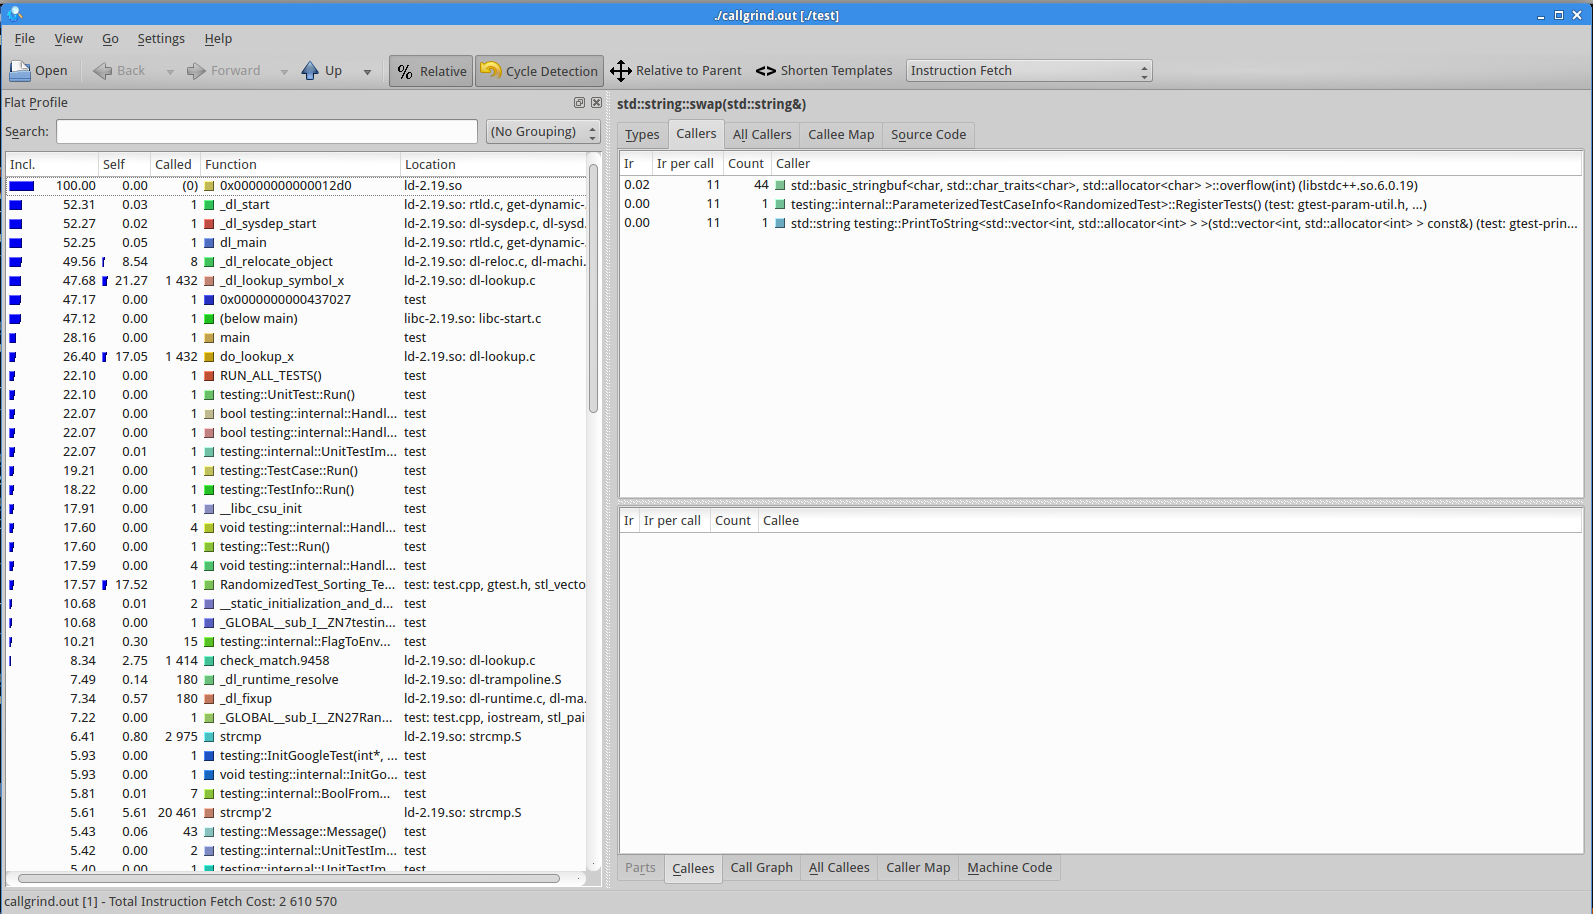
\includegraphics[width=0.8\columnwidth]{kcachegrind.png}
    \caption{Screenshot of the performance details from kcachegrind.}
    \label{fig:kcachegrind}
\end{figure}

\section{Conclusion}
KCachegrind with callgrind and googletest form a fantastic test of tools for
performance regression tests. The Archived reports are sorted in standard
formats such as JUnit, which build servers can use to determine performance
regressions. Automated Matlab or Octave scripts may also part the output to
generate performance trends over time. Also, the beauty of using unit tests as
the key regression functions is they live with the code, and are run with every
build thus regression testing becomes an inseparable part of the continuous
integration and continuous delivery process.

\clearpage
\printbibliography

\end{document}

